\chapter{Úvod}\label{chap:intro}

Tejto úvodnej kapitole by som vás chcel trochu oboznámiť s mojou bakalárkou a poukázať na moju východziu situáciu. Ďalej tiež platformy na ktorých beží a prečo.
\section{Vysvetlenie názvu}
Moja bakalárka sa volá \uv{Optimalizácia obchodovacieho algoritmu na vysoko volatilných komoditných burzách}. Najprv by som tento názov rozobral a podrobne vysvetlil čo to znamená.
\subsection{Optimalizácia obchodného algoritmu}
Vyvíjame algoritmus ktorý bude vedieť sám obchodovať. Mojou úlohou bude tento algoritmus testovať a následne optimalizovať aby podával čo najlepšie výsledky.
\subsection{Vysoko volatilných}
Volatilita\cite{Volatilita} je kolísanie. Miera neistoty. A investíciám je vlastná. Platí, že čím vyššie výnosy, tým vyššia volatilita. Z toho vychádza aj pravidlo investičného horizontu, ktorý je pri rizikovejších – teda volatilnejších – aktívach dlhší. Prečo hľadáme  vysoko volatilné burzy ukážem na príklade.
\subsection{Komoditných burzách}
Náš algoritmus bude pracovať na komoditných burzách konkrétne na burzách pseudo-mien hlavne bitcoin. 

\section{Prečo volatilných?}
Tejto časti sa zameriam na okrajové burzy ktoré sú špecifické svojou vysokou volatilitou
a ukážeme výhody a nevýhody okrajových búrz. A nakoniec zhrnieme prečo nám vyhovujú práve okrajové burzy.
\subsection{Výhody}
\subsubsection{Vysoká volatilita}
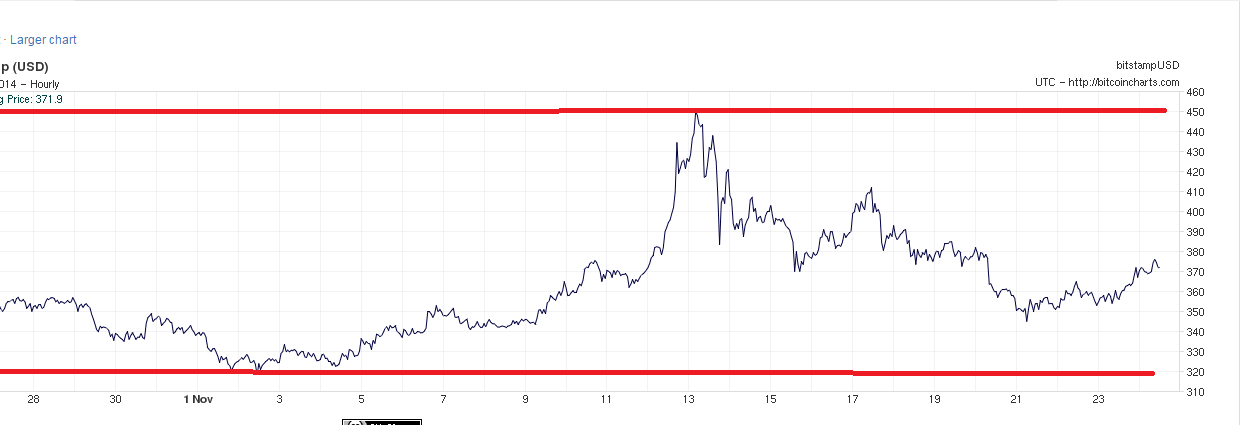
\includegraphics[width=1\textwidth]{obr}
Toto je príklad keď pozeráme na vysoko volatilnú burzu ktorou je bitcoin a USD. Možný zisk sa pohybuje až na úrovni XY percenta. Na rozdiel od ďalšej mále volatilnej burzy kde je  možný zisk iba Z percenta.
\subsubsection{Absencia \uv{Veľkých hráčov}}
\subsection{Nevýhody}
\subsubsection{Veľká likvidita}
\subsubsection{Väčšie riziko}
